%!TEX root = main.tex
\section{Methods\label{sec:methods}}

% Segmentation of ground truth is a labor-intensive, time-consuming process that often needs to be done by reliable workers or experts. There are a few different ways of approaching the segmentation problem. We discuss each of them briefly below.
% \todo[inline]{algorithm-method terminology}
Image annotation problems, and in particular, the segmentation problem can be approached in many ways. In this section we classify and discuss several methods that we use to perform segmentation in images. 
At a broad level, segmentation can be performed using by computer-vision based methods or by using crowdsourcing. We discuss each of these approaches and outline multiple segmentation algorithms below. We evaluate all of these algorithms and report our findings on their performances in Section~\ref{sec:results}.
\todo[inline]{Give names to all methods that can be used in experiments section}
Figure~\ref{flowchart} depicts the classification of approaches as well as the specific algorithms that we will discuss below.

\subsection{Vision-based methods~\label{sec:vision}}
There has been a lot of prior work in segmenting objects based on color boundaries. These approaches, however, are typically non-exact, and far from robust. Furthermore, while they segment the entire image into several disjoint pieces, they do not serve to identify objects. Another class of prior works aim to find rectangular bounding boxes for objects of a specified type, for instance, cars in traffic surveillance images. Our goal, however, is find tight segmentations around specified objects. \dor{the comparison that we made in related works was v.s. specific object segmentation rather than rectangular BB object detection. Maybe we should not talk about rectangular BB to avoid confusion?} Object segmentation using purely automated techniques would require training computer vision models on specific object types. 

We implement a semi-supervised algorithm that can produce segmentations for arbitrary objects in the absence of large volumes of tailor-made training data. While this algorithm works largely on raw image data, it requires some external help in the form of one ``reference'' segmentation. Intuitively, a rough segmentation can be thought of as a pointer for the algorithm to the relevant regions of the image. The algorithm then uses the color profile of the image to segment out the similarly colored regions of the image that overlap with the reference segmentation. Specifically, we begin by splitting the input image into multiple regions, or {\em tiles} that have the same color using the work of~\cite{felzenszwalb2004efficient}---the desired number of output tiles can be modified using a tuning parameter $k$, to produce finer or coarser tiles.\dor{would it be worthwhile to discuss tiles separately at the beginning of section 4 for both aggregation based methods and vision. Or use separate terminology in different the two cases.} Figure~\ref{vision_example} shows one example of the vision color tiling for different chosen granularities. Next, we overlay the given rough segmentation on top of the color tiles. \todo[inline]{img for ref segmentation overlaid on vision tiles (incorporate with Fig.\ref{vision_example})}

\begin{figure}
\vspace{-30pt}
\centering
\begin{subfigure}[b]{\textwidth}
\centering
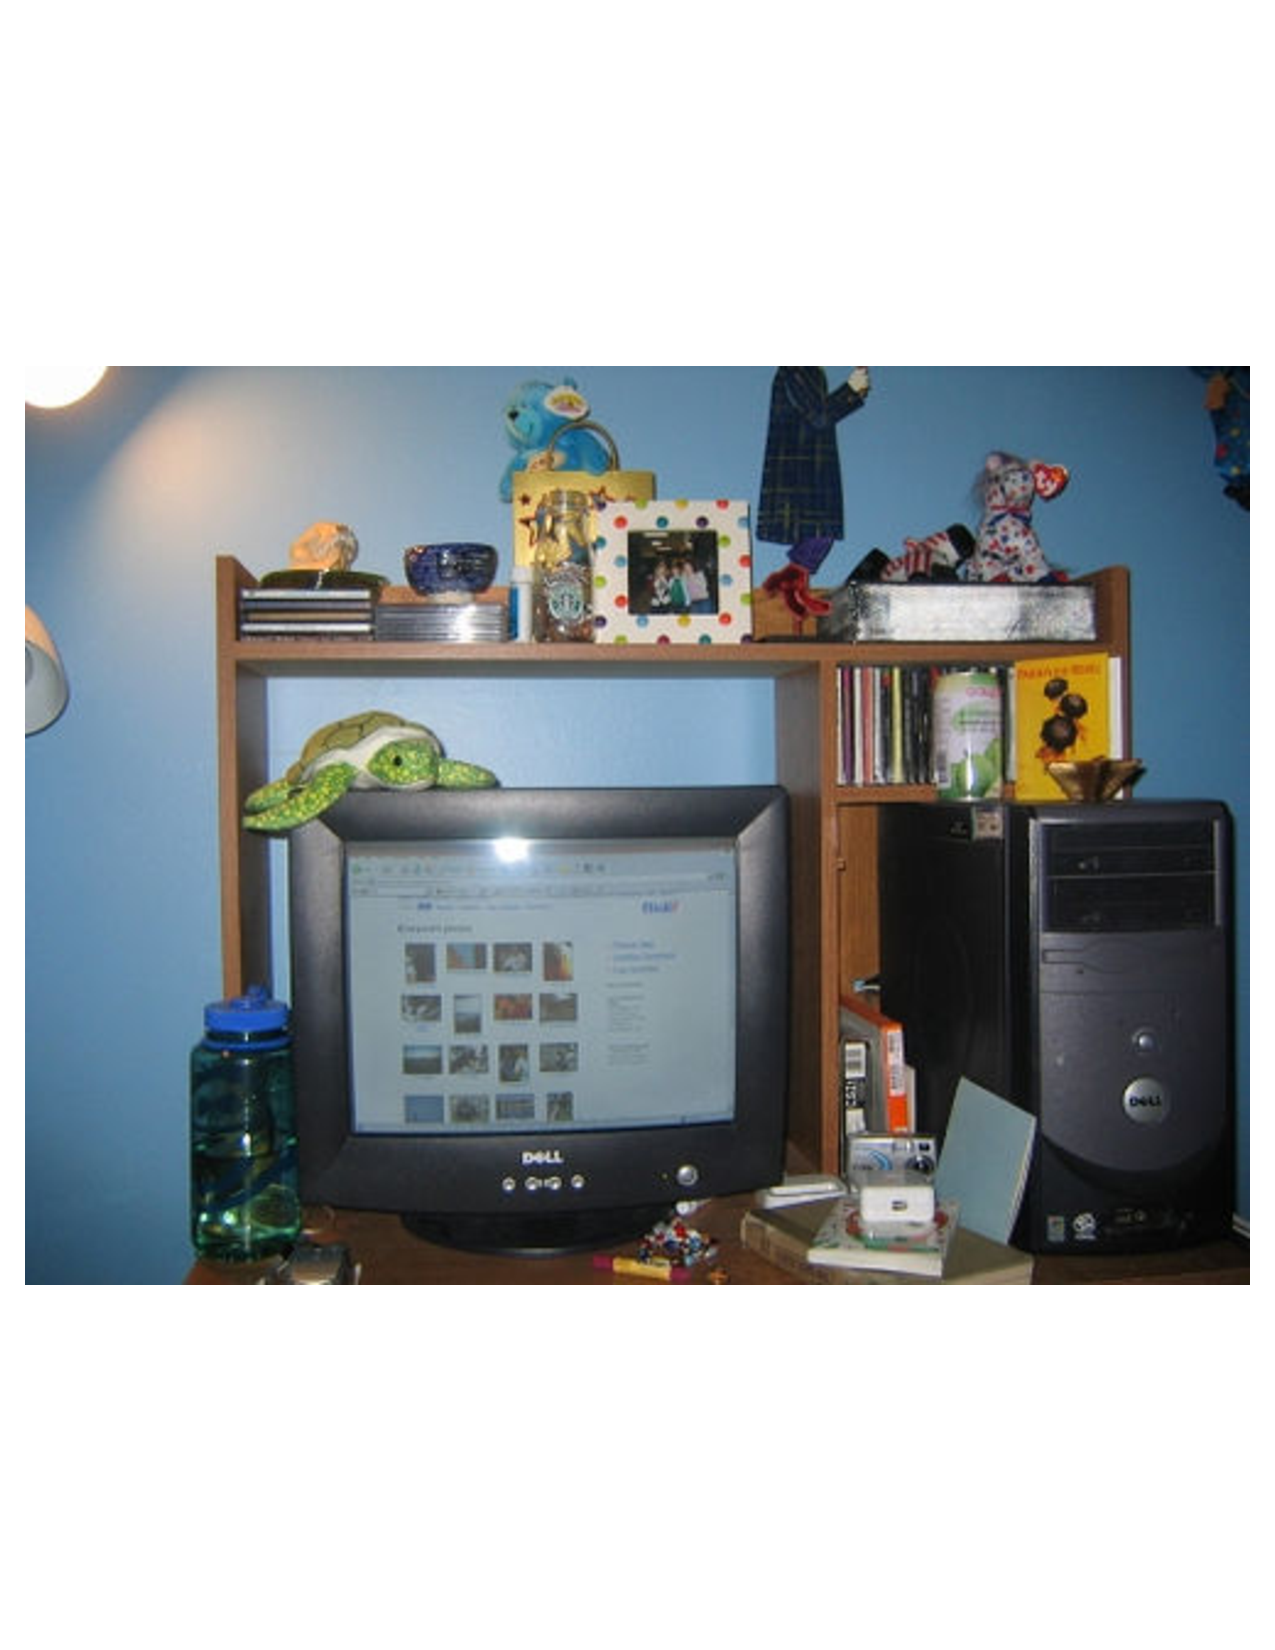
\includegraphics[width=0.7\textwidth]{plots/vision_0.pdf}
\vspace{-70pt}
\end{subfigure}
\begin{subfigure}[b]{\textwidth}
\centering
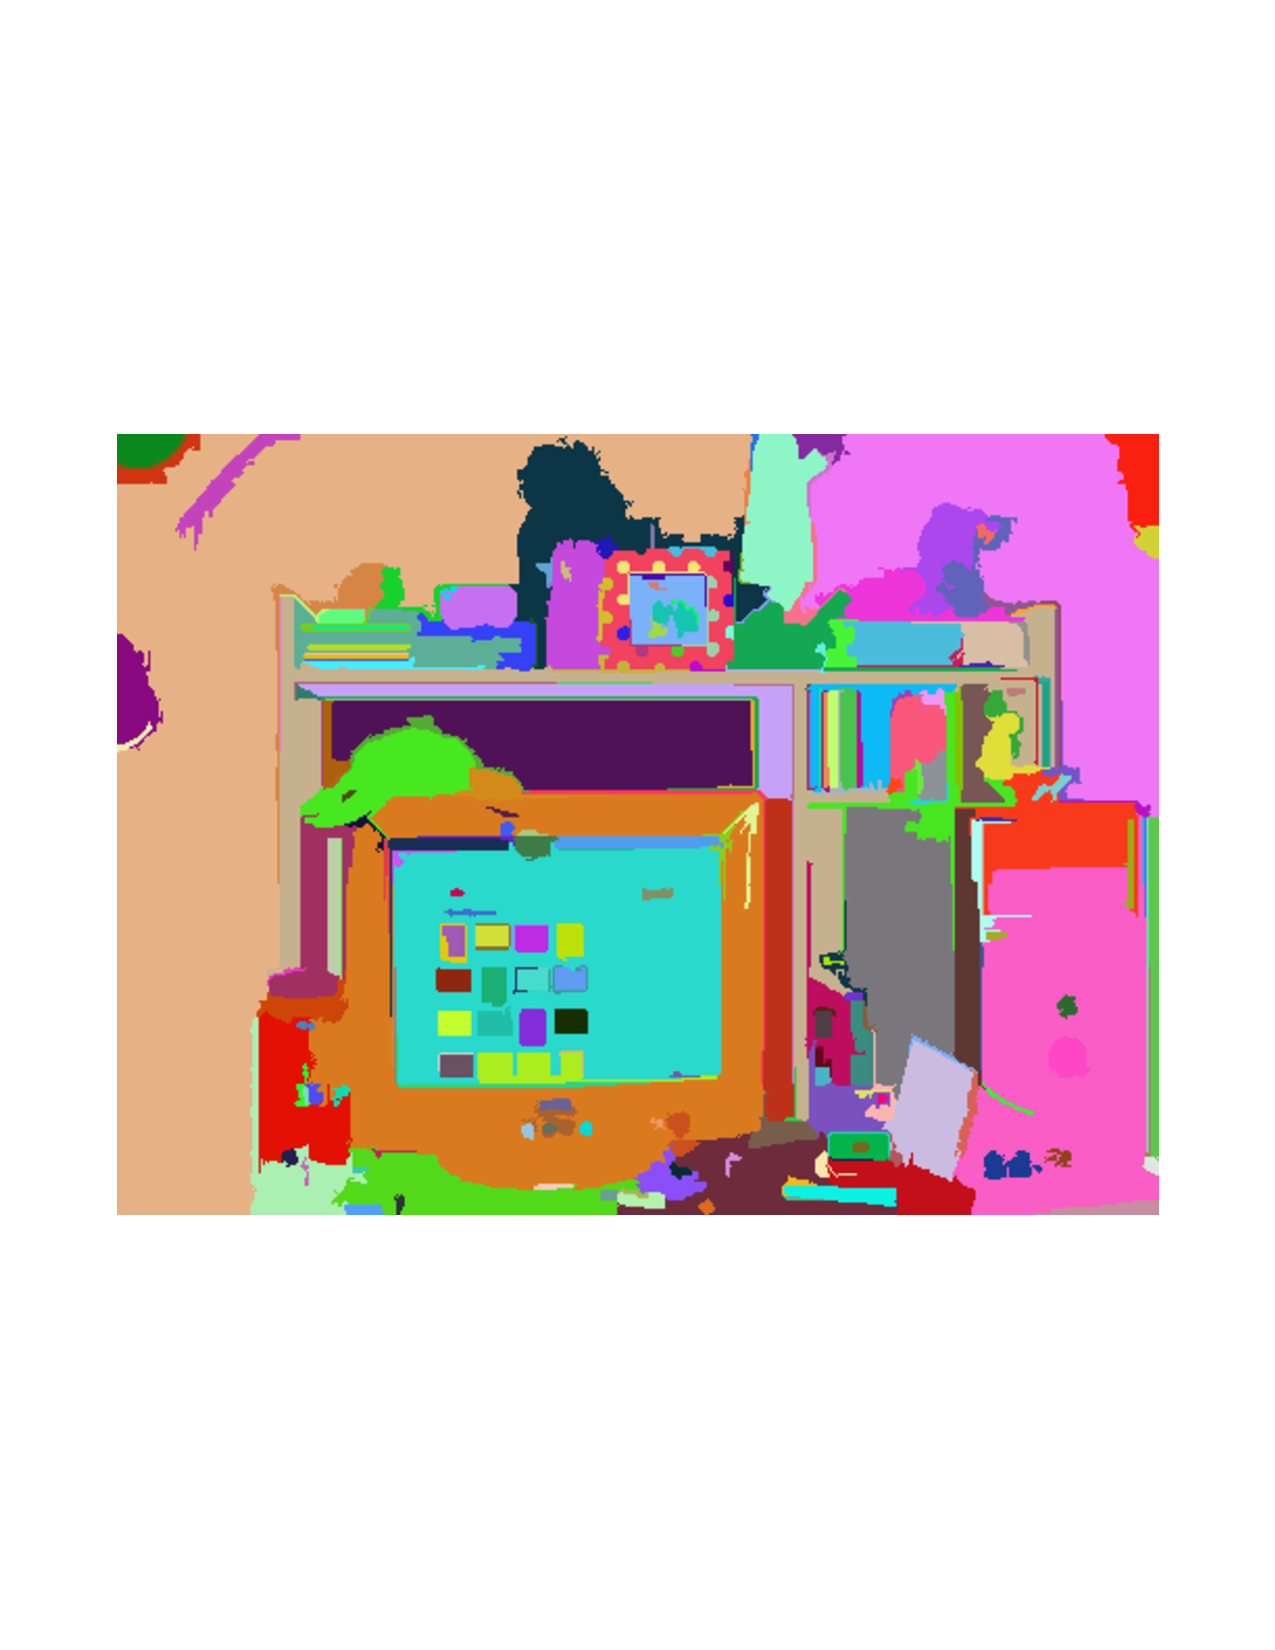
\includegraphics[width=.4\textwidth]{plots/vision_500.pdf}%
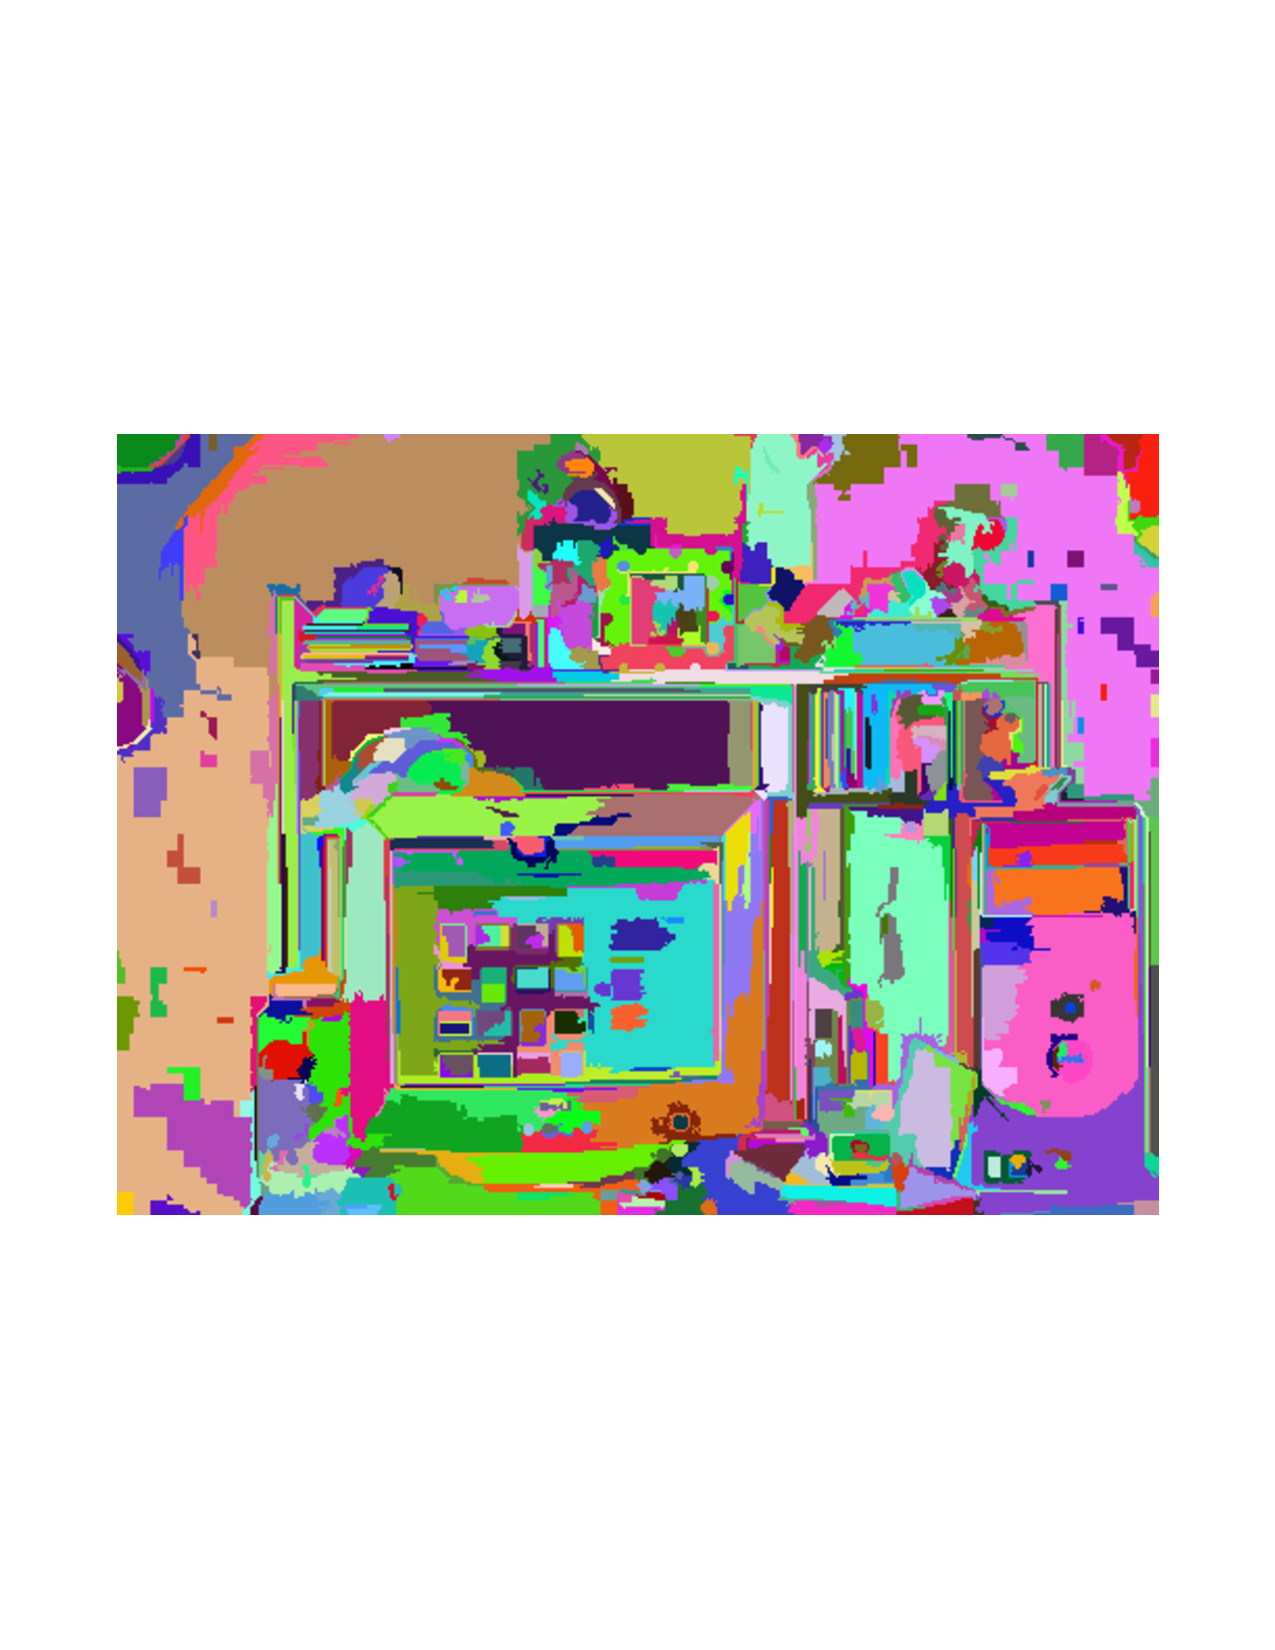
\includegraphics[width=.4\textwidth]{plots/vision_100.pdf}
\vspace{-30pt}
\end{subfigure}
\caption{Left: Raw image. Center: Vision tiles with $k=500$. Right: Vision tiles with $k=100$.}
\label{vision_example}
\end{figure}

Now, the algorithm focuses on {\em choosing the right set of tiles based on the given reference segmentation}. 
Intuitively the algorithm picks color tiles that have significant overlap with the given reference segmentation, i.e., returns the union of all tiles for which greater than a certain area threshold of the tile is intersecting with the reference segmentation. We experiment with different granularities for the vision preprocessing as well as scan a variety of tile filtering area thresholds. 

% \todo[inline]{Vision tile retrieval and vision filling}
We also implemented a second algorithm that looks at this data from the other side, by trying to {\em fix or improve the boundaries of the given reference segmentation using the color tiles information}, discussed in more detail in our technical report.
\techreport{
% begin techreport

\subheading{Color tile retrieval}

\subheading{Segmentation modifying}
Conversely, the second algorithm looks at all the color tiles that have a partial overlap with the given reference object, and then fills in the remainder for tiles that are strongly overlapping with the reference segmentation, and deletes the tiles that have very small overlap with the reference segmentation. 
% end techreport
}

% For each object, we pick parameter that yields the best performing Jaccard.

\subsection{Crowdsourcing methods~\label{sec:crowd}}
Crowdsourcing based approaches use human workers to provide segmentations for objects in images. Since human workers are not perfect and often make mistakes, crowdsourcing approaches typically elicit multiple worker segmentations for each object to reduce output variance resulting from the errors of an individual worker. As we saw in Section~\ref{sec:errors}, different worker segmentations for the same object can differ from each other due to differences in perspective as well as errors in tracing the outline of the object. Crowdsourcing algorithms need to take these multiple differing worker segmentations as input and output a single, accurate segmentation. 

First, we discuss a preprocessing step that helps identify and eliminate the semantic errors (described in Section~\ref{sec:errors}) resulting from multiple perspectives.

\subheading{Worker Clustering}
% \subsection{Clustering~\label{sec:clustering}}
Intuitively, workers that have similar perspectives, will have segmentations that are closer to each other, while workers that have different perspectives from each other will have segmentations that differ from each other. We capture the ``similarity'' of a pair of workers by computing the Jaccard coefficient between their segmentations. We perform {\em spectral clustering} to separate workers, using their pairwise similarities, into clusters. We find that the resulting clusters accurately separate and group workers based on their perspectives or the type of semantic errors they make. We also find that the largest cluster is typically free of any semantic errors. Therefore, our preprocessing step consists of clustering workers based on their mutual pairwise Jaccard similarity scores, and filtering away the workers that do not belong to the largest cluster. %\papertext{\todo[inline]{techreport}We omit the details of the clustering algorithm in the interest of space.}\techreport{\todo[inline]{more details}}

Next, we discuss two classes of crowdsourcing algorithms that fundamentally differ in the way they handle multiple worker segmentations to generate a single output segmentation.

\subheading{Worker retrieval methods}
% \subsection{Retrieval-based~\label{sec:retrieval}}
% The goal of retrieval-based worker is to first evaluate the ``goodness'' of a worker's annotation using annotation scoring functions\cite{Vittayakorn2011}, then retrieve the best 
This class of algorithms tries to identify good and bad workers, and then chooses the best worker segmentation as the output segmentation. In this paper, we look at two different ways of ranking workers and choosing the best worker. First, we use the {\em number of control points}, i.e. number of vertices in a worker's segmentation polygon to rank workers. This is a ranking scheme that~\cite{Vittayakorn2011} showed performs well in practice. Intuitively, workers that have used a larger number of points are likely to have been more precise, and provided a more complex and accurate segmentation. Other heuristic ranking scheme is described in more detail in our technical report~\cite{segmentation-tr}.
\techreport{
% begin techreport
\par Summarization-based metrics are computable heuristics that measure the quality of a worker's bounding box given the ground truth. We employ two metric used in ~\cite{Vittayakorn2011}, number of control points and annotation size, which has been shown to perform better than vision-based summarization metrics. The number of control points metric is based on the intuition that a more precise bounding box consisting of a large number of control points usually indicates that the user made an effort to closely follow the object boundary. The annotation size is based on the intuition that larger bounding-box-to-image-area ratio means that the object is easier to annotate, hence its quality should be higher.
Both of these metrics optimizes for recall at the cost of precision loss.
\par Summarization based metrics does poorly in cases where the 1-D projection of the BBs fails to capture the worker errors fully. They are good indicators assuming the worker error is only based on the degree of sloppiness of his bounding box rather than mistakes on which regions should be incorporated in the object. For the same reasons, these metric also fail in the case of over-bounding or under-bounding BBs. In practice, quality evaluation is done by setting ground truth to be the bounding box with the best summarization score. The upper limit corresponds to the individual worker with the best summarization score when compared against ground truth.
% end techreport    
}
In Section~\ref{sec:agg-detailed} we model worker qualities in terms of their probabilities of annotating pixels of the image correctly, and estimate the worker qualities by utilizing an Expectation-Maximization algorithm. We also use the estimated worker qualities (for different quality models) to predict segmentation accuracy and rank workers, and choose the best worker segmentation based on this ranking as another alternative algorithm.

% We discuss the performances of these and other algorithms in Section~\ref{sec:results}.


\subheading{Aggregation-based methods}
% \subsection{Aggregation-based~\label{sec:aggregation}}
% We are working  with the assumption that we do not have ground truth --- to begin with, therefore use MV or other heuristics to provide a point of comparison, however note that for evaluation purposes the final results cited are always based on comparing with ground truth.
Rather than simply identifying and picking a single worker's segmentation, aggregation-based methods seek to combine multiple workers' segmentations into a single merged segmentation. At the heart of all our aggregation techniques is the following data representation: we logically overlay all workers' segmentations on top of each other within the framework of the overall image. As illustrated in \ref{tile_demo}, the overlaid worker segmentations can be thought of as a Venn diagram that represents a partitioning of the entire image into multiple worker {\em tiles} formed by the intersections of different worker segmentations. We then choose and merge a subset of the tiles to give the final output segmentation\dor{vague}. The intuition here is that by splitting the image into tiles, we get finer granularity information than by looking at complete segmentations. This also allows us to aggregate data from multiple workers rather than having to choose a single worker bounding box---this allows for the potential of choosing the best partial segmentations for an object and joining them, or fixing one worker's errors by taking the help of another worker's segmentation. The problem of choosing a good set of tiles is, however, non-trivial.
Since aggregation based methods are the least studied methods by previous work, we discuss them in further detail in Section~\ref{sec:agg-detailed}.
